\documentclass[10pt,c,aspectratio=1610,handout]{beamer}
\usetheme[block=fill,numbering=fraction,progressbar=frametitle]{metropolis}
%\usecolortheme{beaver}
\usepackage{textpos}
\usepackage{amsmath}
\usepackage{amssymb}
\usepackage{hyperref}
\usepackage{appendixnumberbeamer}

\setbeamercovered{transparent}

\newcommand\blfootnote[1]{%
  \begingroup
  \renewcommand\thefootnote{}\footnote{#1}%
  \addtocounter{footnote}{-1}%
  \endgroup
}

\renewcommand{\baselinestretch}{1.25}
% Colour theme
\definecolor{QDMblue}{rgb}{0.00, 0.1882, 0.3608}
\definecolor{QDMgold}{rgb}{0.9098, 0.6510, 0.0000}
\definecolor{QDMgreen}{rgb}{0.3098, 0.5490, 0.0510}
\setbeamercolor{normal text}{ fg= QDMblue , bg= white }
\setbeamercolor{alerted text}{ fg= QDMgold }
\setbeamercolor{example text}{ fg= QDMgreen }

\begin{document}

% Personal Info
\title{Introduction to Modern Macroeconomics}
\author[Konstantin Gantert]{\begin{large} Konstantin Gantert \end{large} \\ \textbf{Quantitative Dynamic Macroeconomics}}
\date{\textit{this version:} \today}

% Eliminates Navigation Bar on every Frame
\beamertemplatenavigationsymbolsempty

%-------------------------------------------------------------------------
% 0.1 Titlepage
%-------------------------------------------------------------------------
{\setbeamertemplate{footline}{} 
\frame{\titlepage}}
 \addtocounter{framenumber}{-1}
%-------------------------------------------------------------------------
% ABOUT THE COURSE
%-------------------------------------------------------------------------

% Course Learning Goals
\begin{frame}{Course Learning Goals}%
  After \emph{successful completion of the course}, the student will be able to:%
  \vspace{0.1in}%
  \pause%
  \begin{itemize}%
    \item[\textbf{CG 1}] implement the structure of macroeconomic research papers, especially of model-based quantitative research papers.%
    \pause%
    \item[\textbf{CG 2}] illustrate how the assumptions of "Dynamic Stochastic General Equilibrium" models define the model environment and its outcomes.%
    \pause%
    \item[\textbf{CG 3}] apply mathematical methods to solve macroeconomic models described by systems of linear difference equations.%
    \pause%
    \item[\textbf{CG 4}] compute software-based simulations, statistics, and visualizations of "Dynamic Stochastic General Equilibrium" models.%
    \pause%
    \item[\textbf{CG 5}] organize the building blocks of "Dynamic Stochastic General Equilibrium" models such as Real-Business-Cycle and New-Keynesian models.%
    \pause%
    \item[\textbf{CG 6}] assess economic transmission channels and policy based on computer simulations of ''Dynamic Stochastic General Equilibrium'' models.%
  \end{itemize}%
\end{frame}%
%-------------------------------------------------------------------------
% Table of Contents for the Course
\begin{frame}[c]{Table of Contents for the Course}%
  \begin{minipage}{0.475\textwidth}%
    \textbf{Block 1: The Basics of DSGE Models}%
    \vspace{0.1in}%
    \begin{enumerate}%
      \item[1.] Introduction to Modern Macro%
      \item[2.] A Dynamic Cash-in-Advance Economy%
      \item[3.] Shocks and the Statistical Model%
    \end{enumerate}%
    \vspace*{0.1in}%
    \pause%
    \textbf{Block 2: Expanding the CiA Model}%
    \vspace*{0.1in}%
    \begin{enumerate}
      \item[4.] Monetary Policy and Inflation%
      \item[5.] Capital and Fiscal Policy%
      \item[6.] Solving a Fully Dynamic CiA Model%
    \end{enumerate}
  \end{minipage}%
  \hfill%
  \pause%
  \begin{minipage}{0.475\textwidth}%
    \textbf{Block 3: Policy Analysis (Term Paper)}%
    \vspace{0.1in}%
    \begin{enumerate}%
      \item[7.] New-Keynesian Business Cycle Model%
      \item[8.] Discussion Workshop%
      \item[9.] Open Room \& Coding Impulse%
      \item[10.] Open Room \& Coding Impulse%
      \item[11.] Open Room \& Coding Impulse%
      \item[12.] Open Room \& Coding Impulse%
      \item[13.] Open Room \& Peer Feedback%
      \item[14.] Term Paper Deadline%
    \end{enumerate}%
  \end{minipage}%
\end{frame}%
%-------------------------------------------------------------------------

% Outline for this Lecture
\begin{frame}{Outline for this Lecture}%
  \onslide<1->{
  \begin{minipage}{0.48\textwidth}%
    \textbf{What you have seen before}%
    \begin{small}%
    \begin{enumerate}%
      \item National accounting%
      \item AS-AD(IS-MP) model%
      \item Solow growth model%
      \item Lagrange method%
    \end{enumerate}%
    \end{small}%
  \end{minipage}}%
  \onslide<3->{
  \hfill%
  \begin{minipage}{0.48\textwidth}%
    \textbf{What you will see today}%
    \begin{small}%
    \begin{enumerate}%
      \item Macro data \& AS-AD short-comings {\tiny[CG 1]}%
      \item Macro policy in practice {\tiny[CG 6]}%
      \item Discussion of assignment 0 {\tiny[CG 1, 5]}%
      \item Static CiA macroeconomic model {\tiny[CG 1, 5]}%
    \end{enumerate}%
    \end{small}%
  \end{minipage}}%
  \vspace*{0.25in}%
  \onslide<2->{
  \begin{block}{Big Picture of the Lecture}%
    \begin{enumerate}%
      \item Why do we need dynamic macroeconomic models to explain business cycle fluctuations?%
      \item How do we go from microeconomics to aggregate macroeconomic models?%
    \end{enumerate}%
  \end{block}}%
\end{frame}%
%-------------------------------------------------------------------------
% BLOCK 1 - Motivation: Why do we need Dynamic Macroeconomic Models?
%-------------------------------------------------------------------------
\section{Motivation:\\\small{Why do we need Dynamic Macroeconomic Models?}}
%-------------------------------------------------------------------------
% Dynamic Patterns: Long-Term Growth and Short-Term Fluctuation
\begin{frame}{Dynamic Patterns: Long-Term Growth and Short-Term Fluctuation}%
  \begin{minipage}{0.5\textwidth}%
    \begin{figure}%
      \centering%
      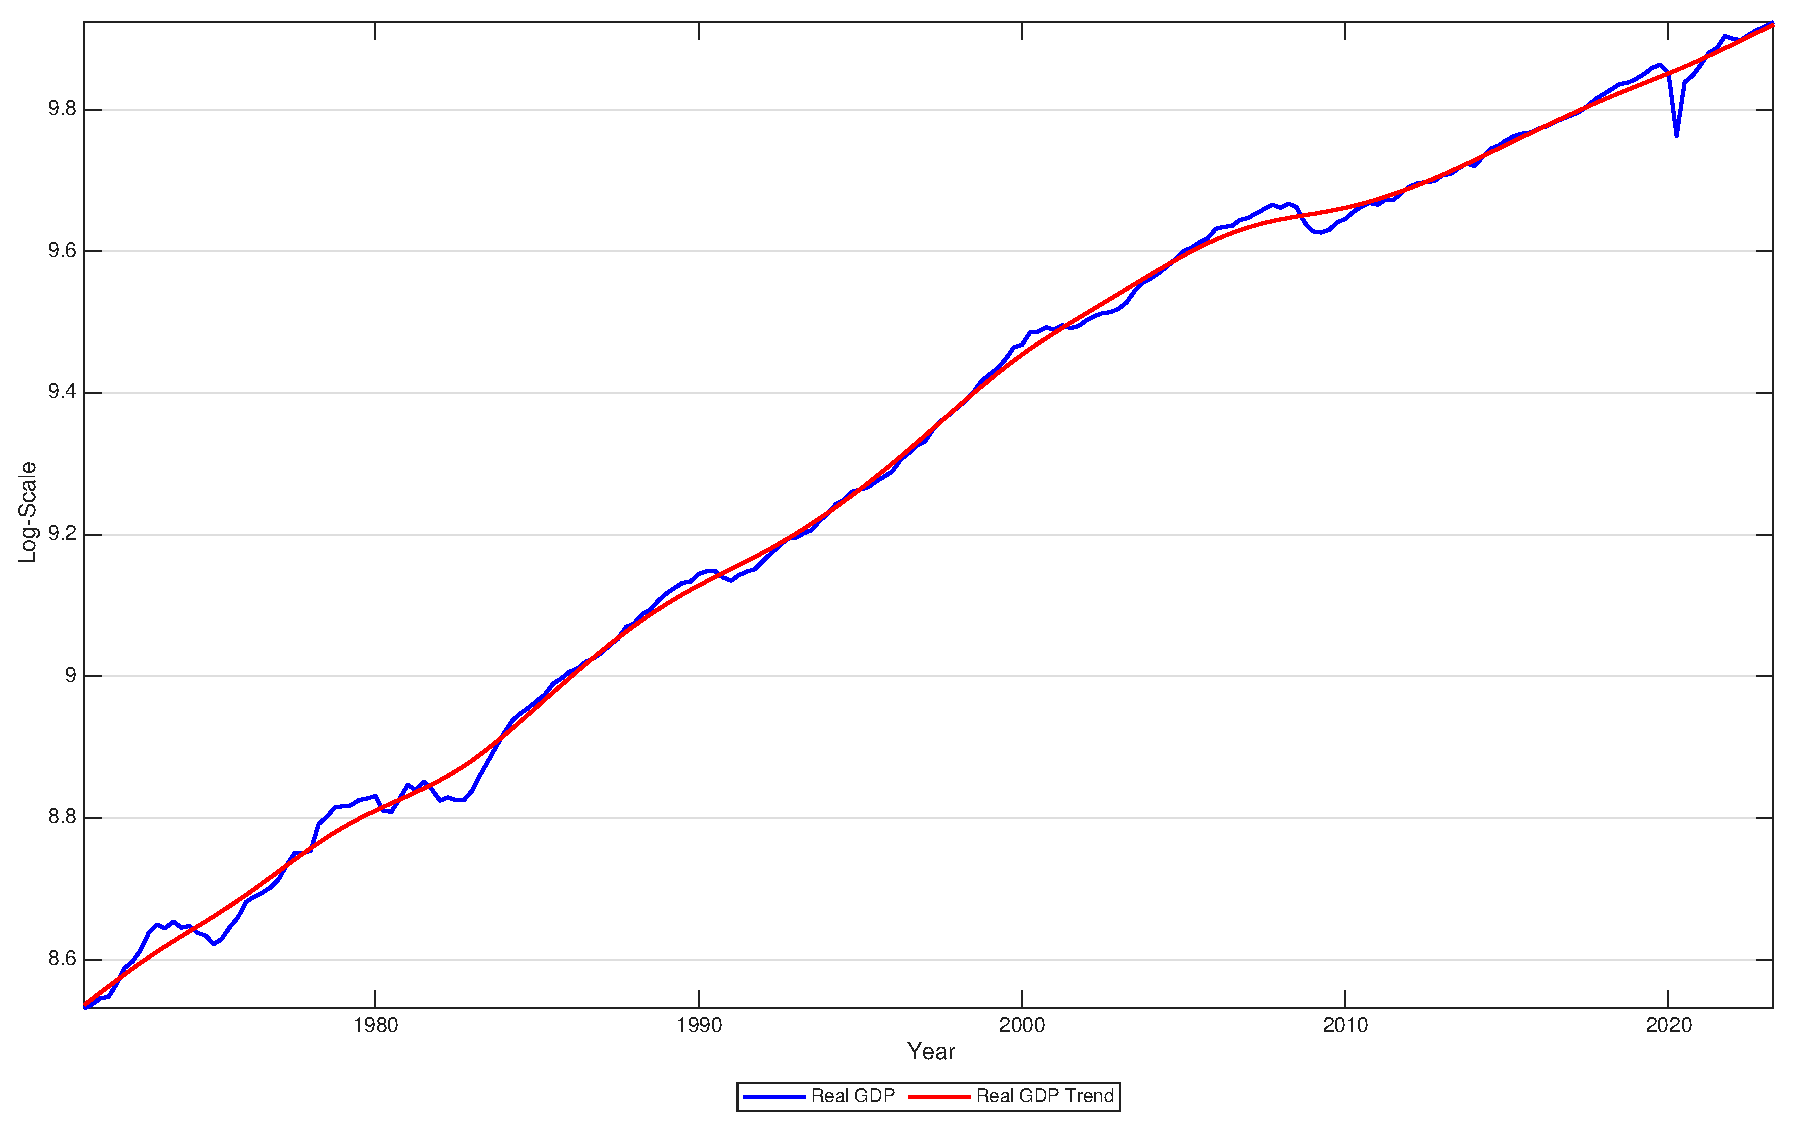
\includegraphics[width=\linewidth]{figures/gdp_growth.eps}%
      \vspace*{-0.1in}%
      \caption{Real GDP in the US (1980-2023)}%
      \vspace*{-0.5in}%
    \end{figure}%
  \end{minipage}%
  \hfill%
  \pause%
  \begin{minipage}{0.47\textwidth}%
    \begin{small}%
      \textbf{Some real GDP growth statistics:}%
      \begin{itemize}%
        \item[$\blacktriangleright$] Average growth rate: $2.56 \%$%
        \item[$\blacktriangleright$] Autocorrelation (trend growth):%
        \begin{itemize}%
          \item 1-period lag: $0.99$%
          \item 8-period lag: $0.76$%
          \item 16-period lag: $0.35$%
        \end{itemize}%
      \end{itemize}%
      \vspace*{0.2in}%
      \pause%
      \textbf{How to describe the growth patterns?}%
      \begin{itemize}%
        \item[$\blacktriangleright$] We need a model that makes time explicitly in the long-run.%
        \item[$\blacktriangleright$] Solow growth model!%
        \item[$\blacktriangleright$] But what about the short-run and microfoundations?%
      \end{itemize}%
    \end{small}%
  \end{minipage}%
\end{frame}%
%-------------------------------------------------------------------------
% Dynamic Patterns: The Business Cycle - Booms and Busts
\begin{frame}{Dynamic Patterns: The Business Cycle - Booms and Busts}%
  \begin{minipage}{0.5\textwidth}%
    \begin{figure}%
      \centering%
      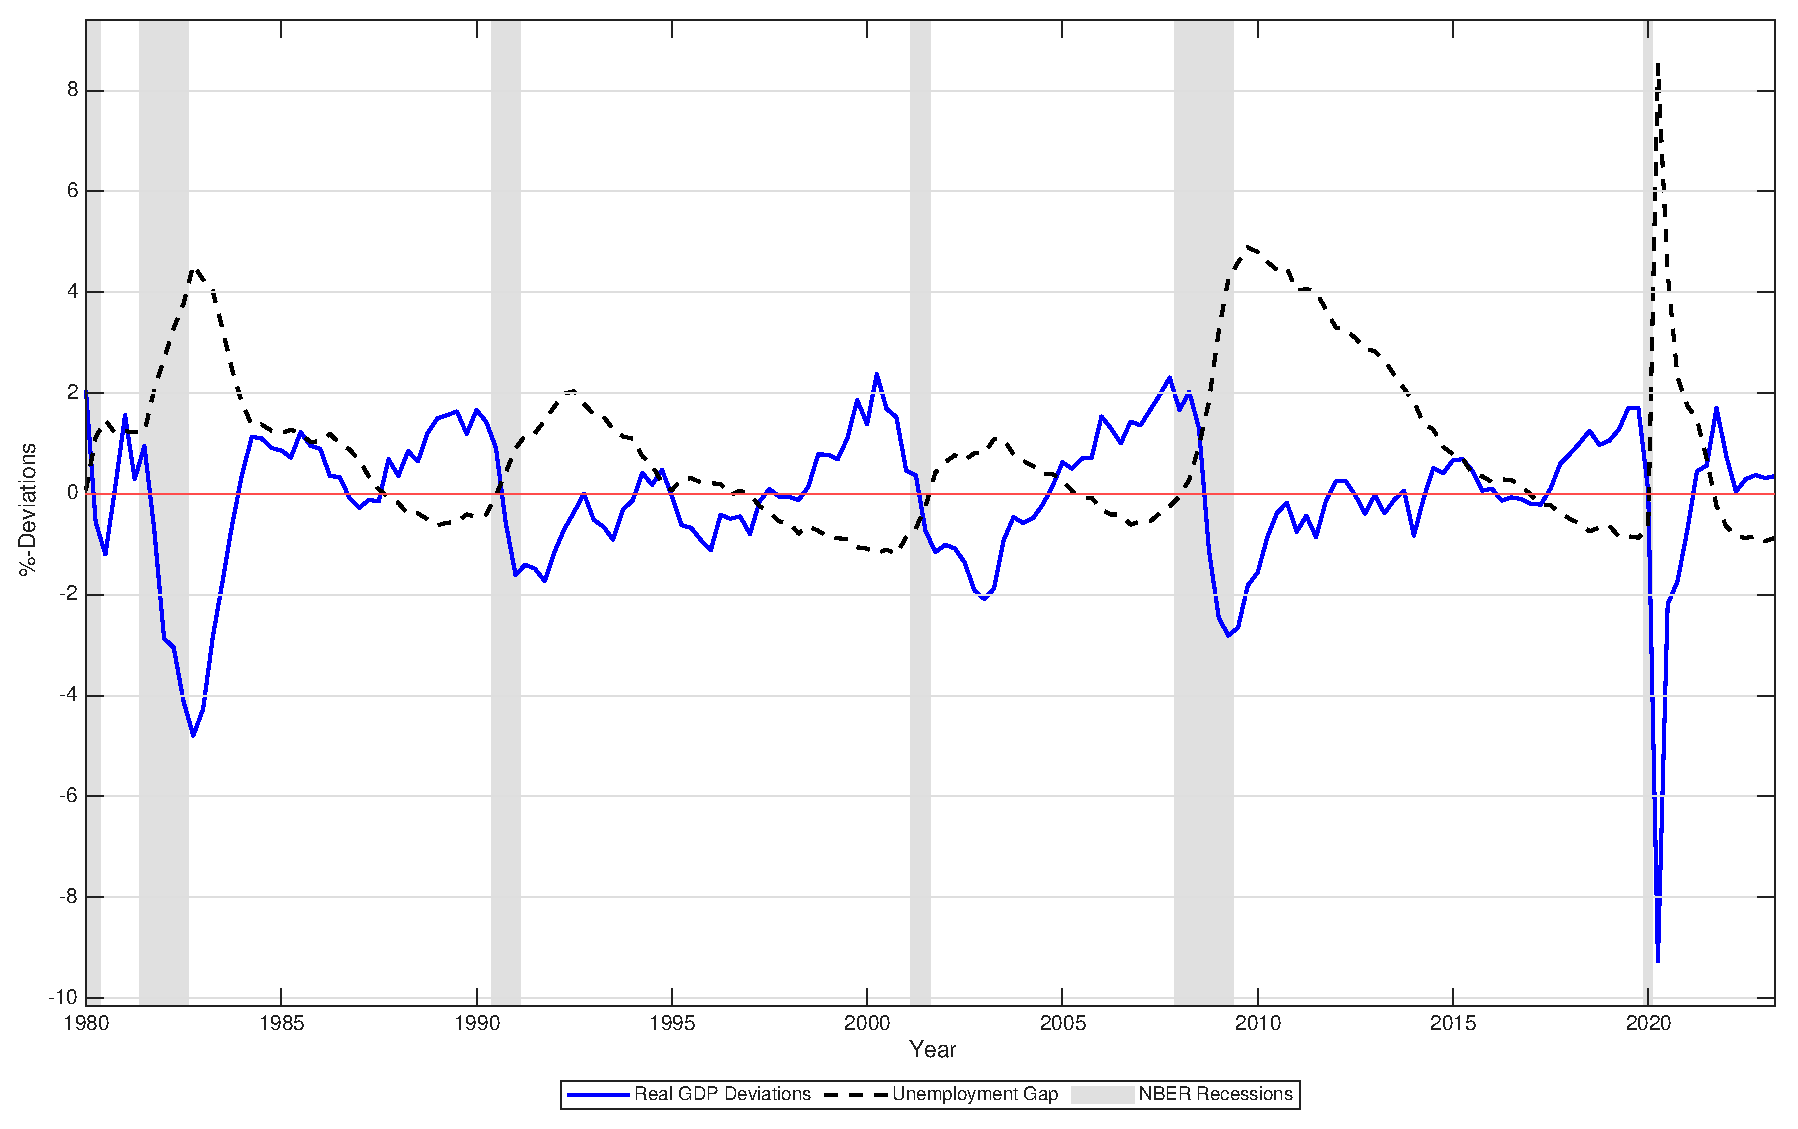
\includegraphics[width=\linewidth]{figures/gdp_cycle.eps}%
      \vspace*{-0.1in}%
      \caption{Quarterly Real GDP Deviations from the Long-Term Trend in the US (1980-2023)}%
      \vspace*{-0.5in}%
    \end{figure}%
  \end{minipage}%
  \hfill%
  \pause%
  \begin{minipage}{0.47\textwidth}%
    \begin{small}%
      \textbf{Some business cycle statistics:}%
      \begin{itemize}%
        \item[$\blacktriangleright$] Standard deviation: 
        \begin{itemize}%
          \begin{small}%
            \item $1.43 \%$ (GDP); $1.63 \%$ (UE)%
          \end{small}%
        \end{itemize}%
        \item[$\blacktriangleright$] Autocorrelation (Quarters):%
        \begin{itemize}%
          \begin{small}%
            \item 1-lag: $0.70$ (GDP); $0.87$ (UE)%
            \item 2-lag: $0.49$ (GDP); $0.77$ (UE)%
            \item 3-lag: $0.30$ (GDP); $0.68$ (UE)%
          \end{small}%
        \end{itemize}%
      \end{itemize}%
      \vspace*{0.2in}%
      \pause%
      \textbf{How to describe the fluctuations?}%
      \begin{itemize}%
        \item[$\blacktriangleright$] AS-AD model? Does not show dynamics - only short- and long-run!%
        \item[$\blacktriangleright$] We need a model that makes time explicit in the short-run.%
      \end{itemize}%
    \end{small}%
  \end{minipage}%
\end{frame}%
%-------------------------------------------------------------------------
% Microfoundations: Inflation and Unemployment: The Phillips Curve
\begin{frame}{Microfoundations: Inflation and Unemployment - The Phillips Curve}%
  \begin{minipage}{0.5\textwidth}%
    \vspace{0.1in}%
    \begin{figure}%
      \centering%
      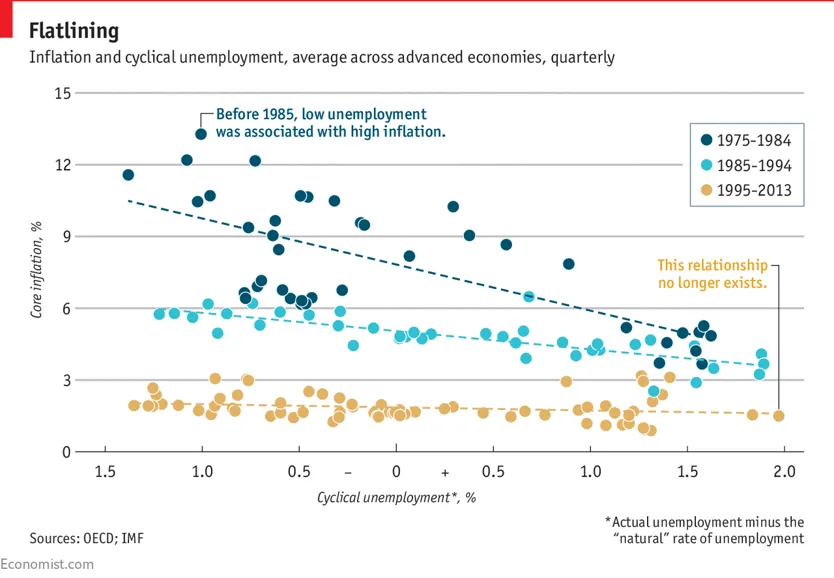
\includegraphics[width=0.7\linewidth]{figures/phillips_curve_economist.png}\\%
      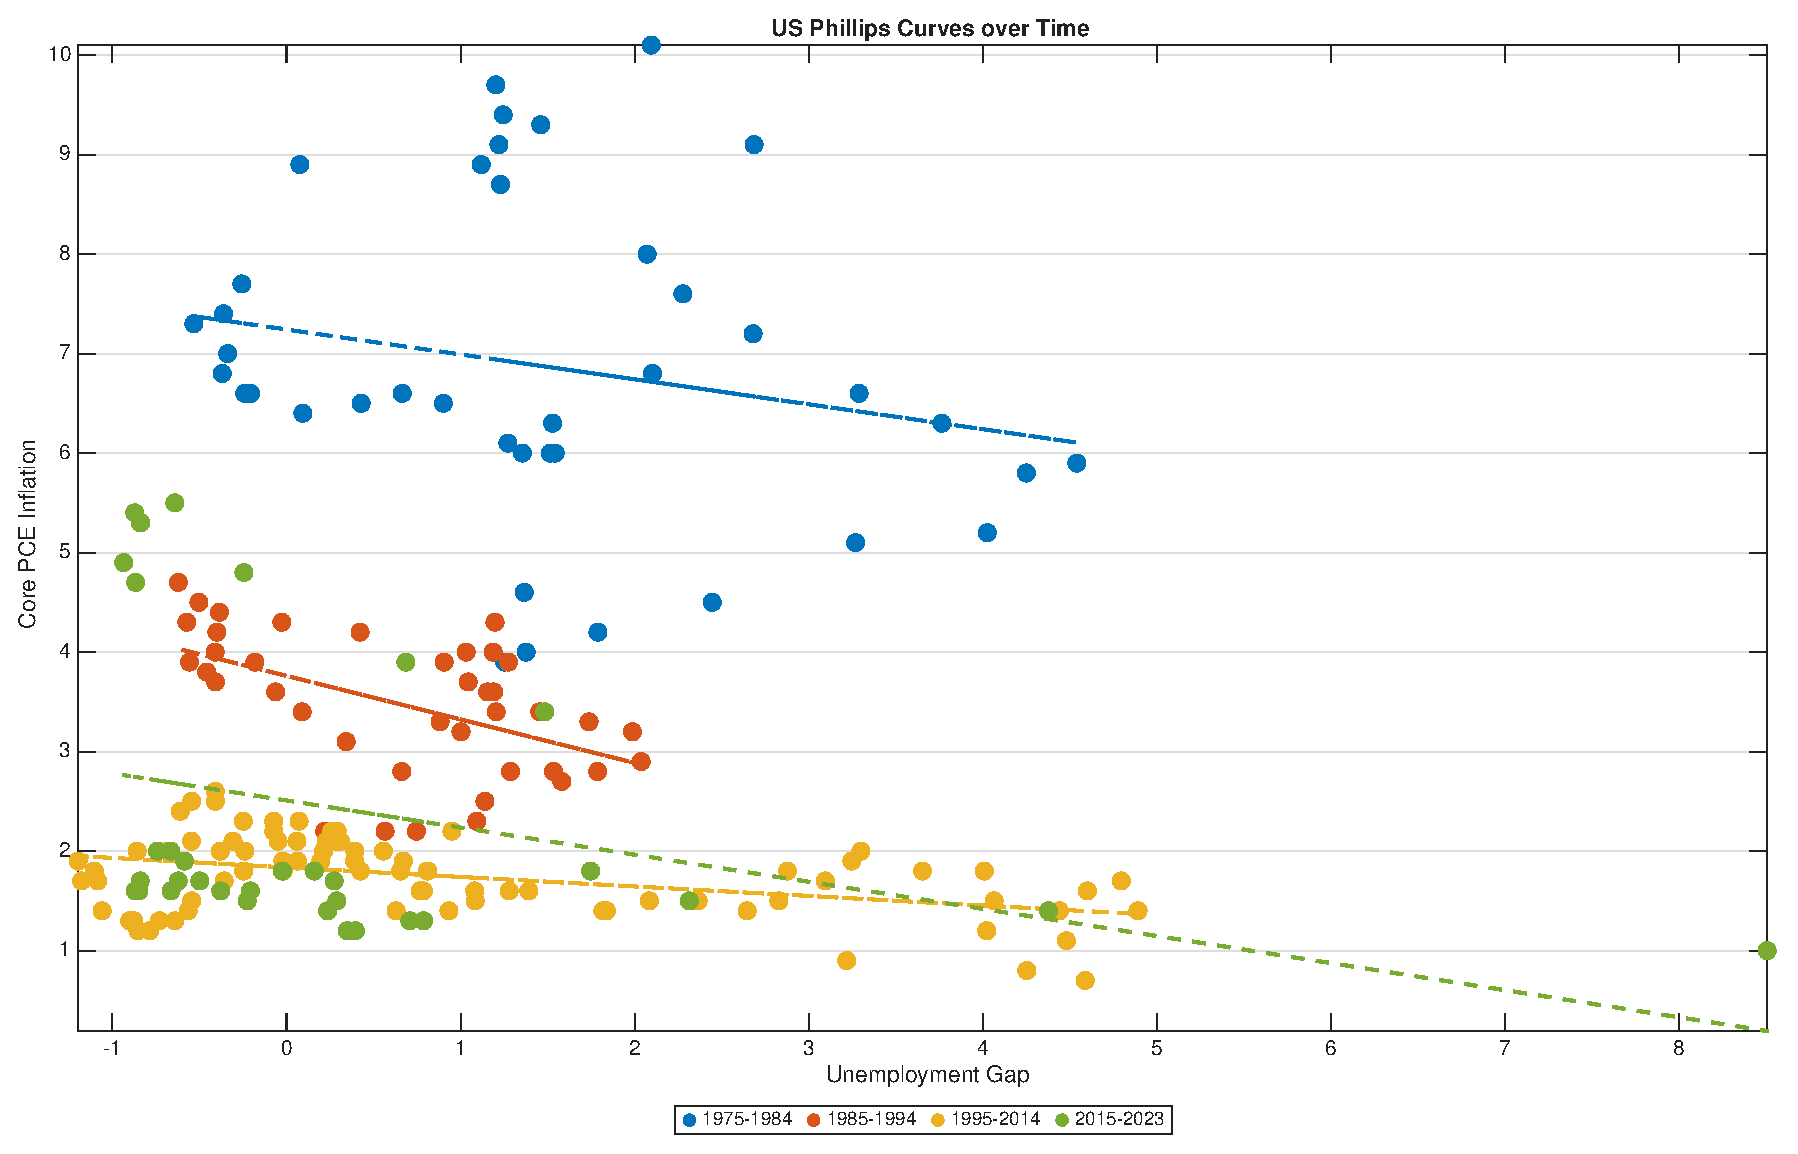
\includegraphics[width=0.7\linewidth]{figures/phillips_us.eps}%
      \vspace{-0.25in}%
      \caption{The flattening of the Phillips curve (top: \emph{The Economist}; bottom: own, FRED)}%
    \end{figure}%
  \end{minipage}%
  \hfill%
  \pause%
  \begin{minipage}{0.47\textwidth}%
    \begin{small}%
      \textbf{Can we derive (aggregate) decision rules from the data?}%
      \begin{itemize}%
        \item[$\blacktriangleright$] Phillips (1958) shows a statistical pattern between inflation and unemployment.%
        \item[$\blacktriangleright$] The AS-AD model uses such statistical relationships as fundamental equations.%
        \pause%
        \item[$\blacktriangleright$] What if underlying institutions, preferences, or technologies change?%
        \item[$\blacktriangleright$] Is this how agents behave? Or should we base our decisions on micro-foundations?%
      \end{itemize}%
    \end{small}%
  \end{minipage}%
\end{frame}%
%-------------------------------------------------------------------------
% Microfoundations: The Impact of Inflation Expectations
\begin{frame}{Microfoundations: The Impact of Inflation Expectations}%
  \begin{minipage}{0.5\textwidth}%
    \begin{figure}%
      \centering%
      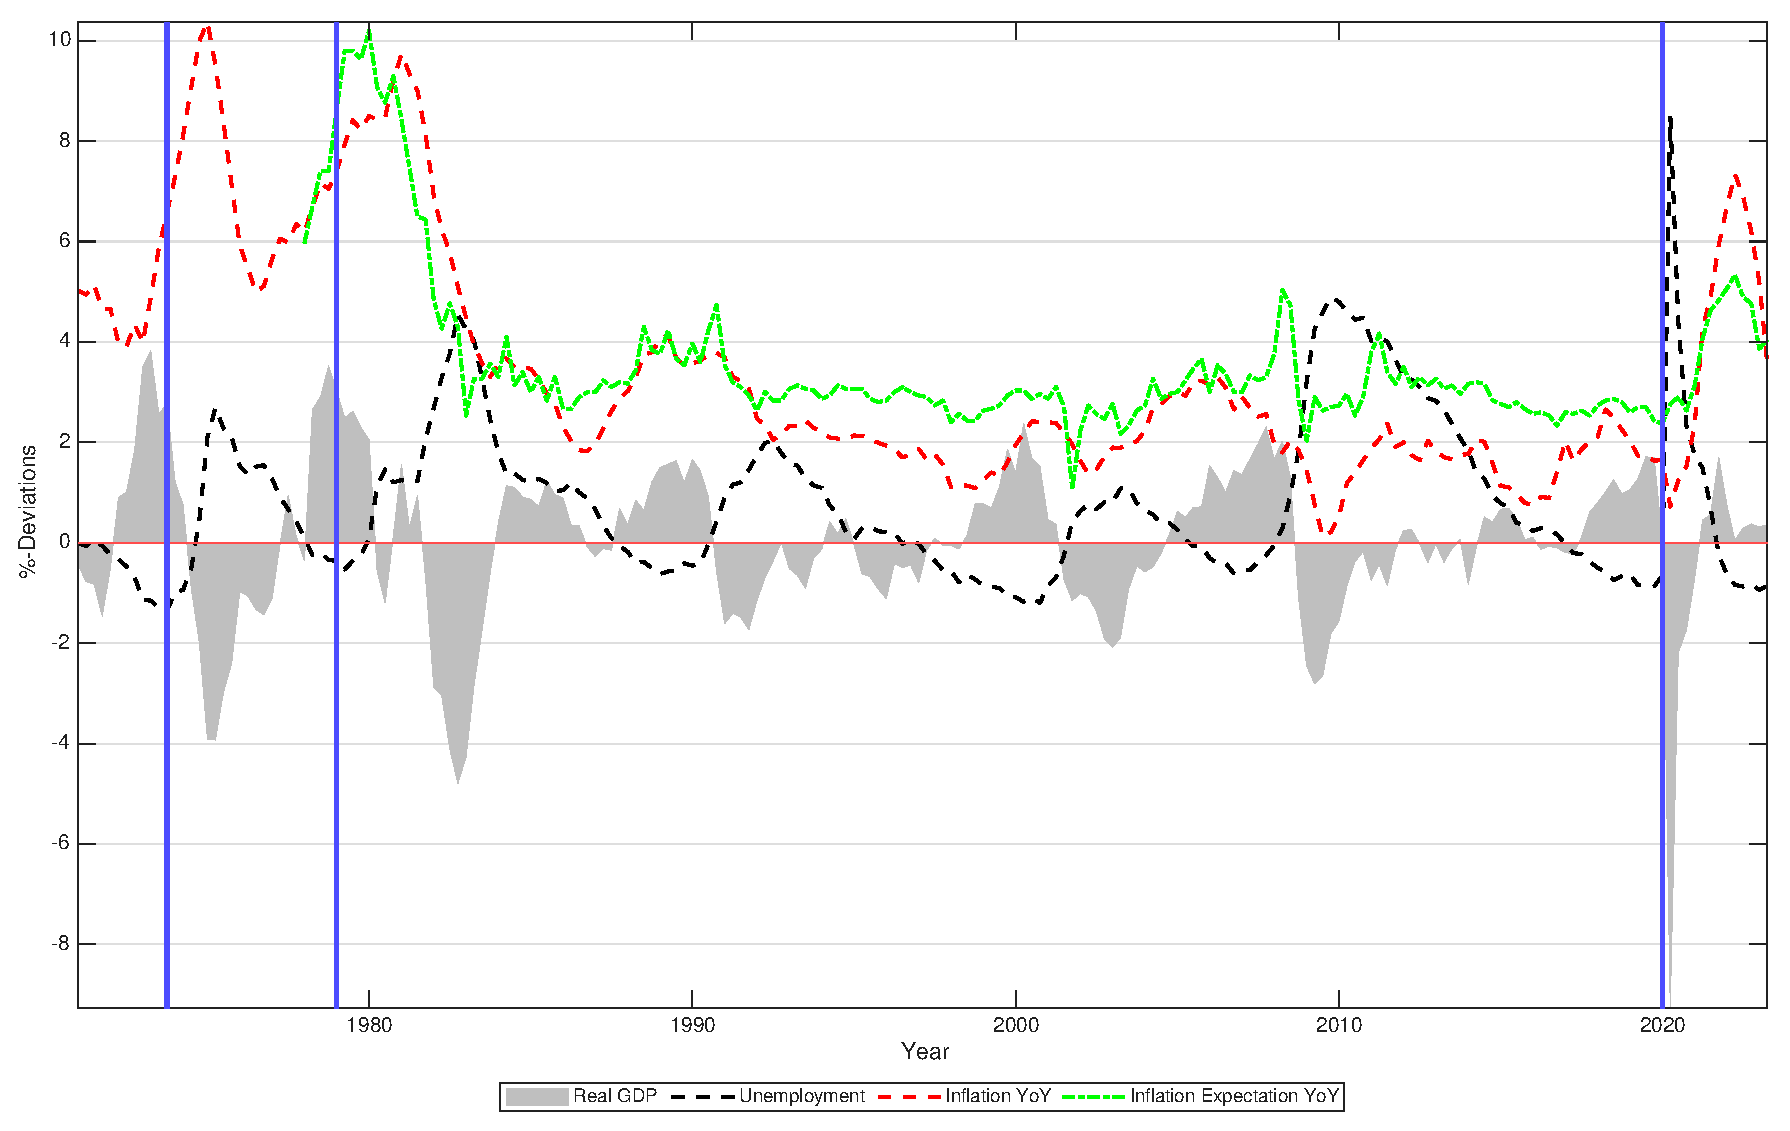
\includegraphics[width=\textwidth]{figures/infl_exp.eps}%
      \vspace*{-0.1in}%
      {\small \caption{Fluctuations in real GDP and inflation expectations as drivers of inflation for US quarterly data (1980-2023).}}%
      \vspace*{-0.5in}%
    \end{figure}%
  \end{minipage}%
  \hfill%
  \pause%
  \begin{minipage}{0.47\textwidth}%
    \begin{small}%
      A typical \textbf{Phillips curve}: $$\pi = \kappa \times \tilde{GDP} + \xi + \pi_E$$%
      \vspace*{-0.25in}%
      \begin{itemize}
        \item[$\rightarrow$] What determines expectations, $\pi_E$?%
      \end{itemize}
      \vspace*{0.15in}%
      \pause%
      \textbf{Expectation formation:}%
      \begin{itemize}%
        \item[$\blacktriangleright$] Agents observe the past and form expectations about the future.%
        \item[$\blacktriangleright$] How do agents form expectations about the future?%
        \begin{itemize}%
          \item[$\rightarrow$] Rational expectations%
          \item[$\rightarrow$] Adaptive expectations%
        \end{itemize}%
      \end{itemize}%
    \end{small}%
  \end{minipage}%
\end{frame}%
%-------------------------------------------------------------------------
% Stochastic Elements: How to model Expectations about Natural Disasters?
\begin{frame}{Stochastic Elements: How to model Expectations about Natural Disasters?}%
  \begin{minipage}{0.5\textwidth}%
    \begin{figure}
      \centering
      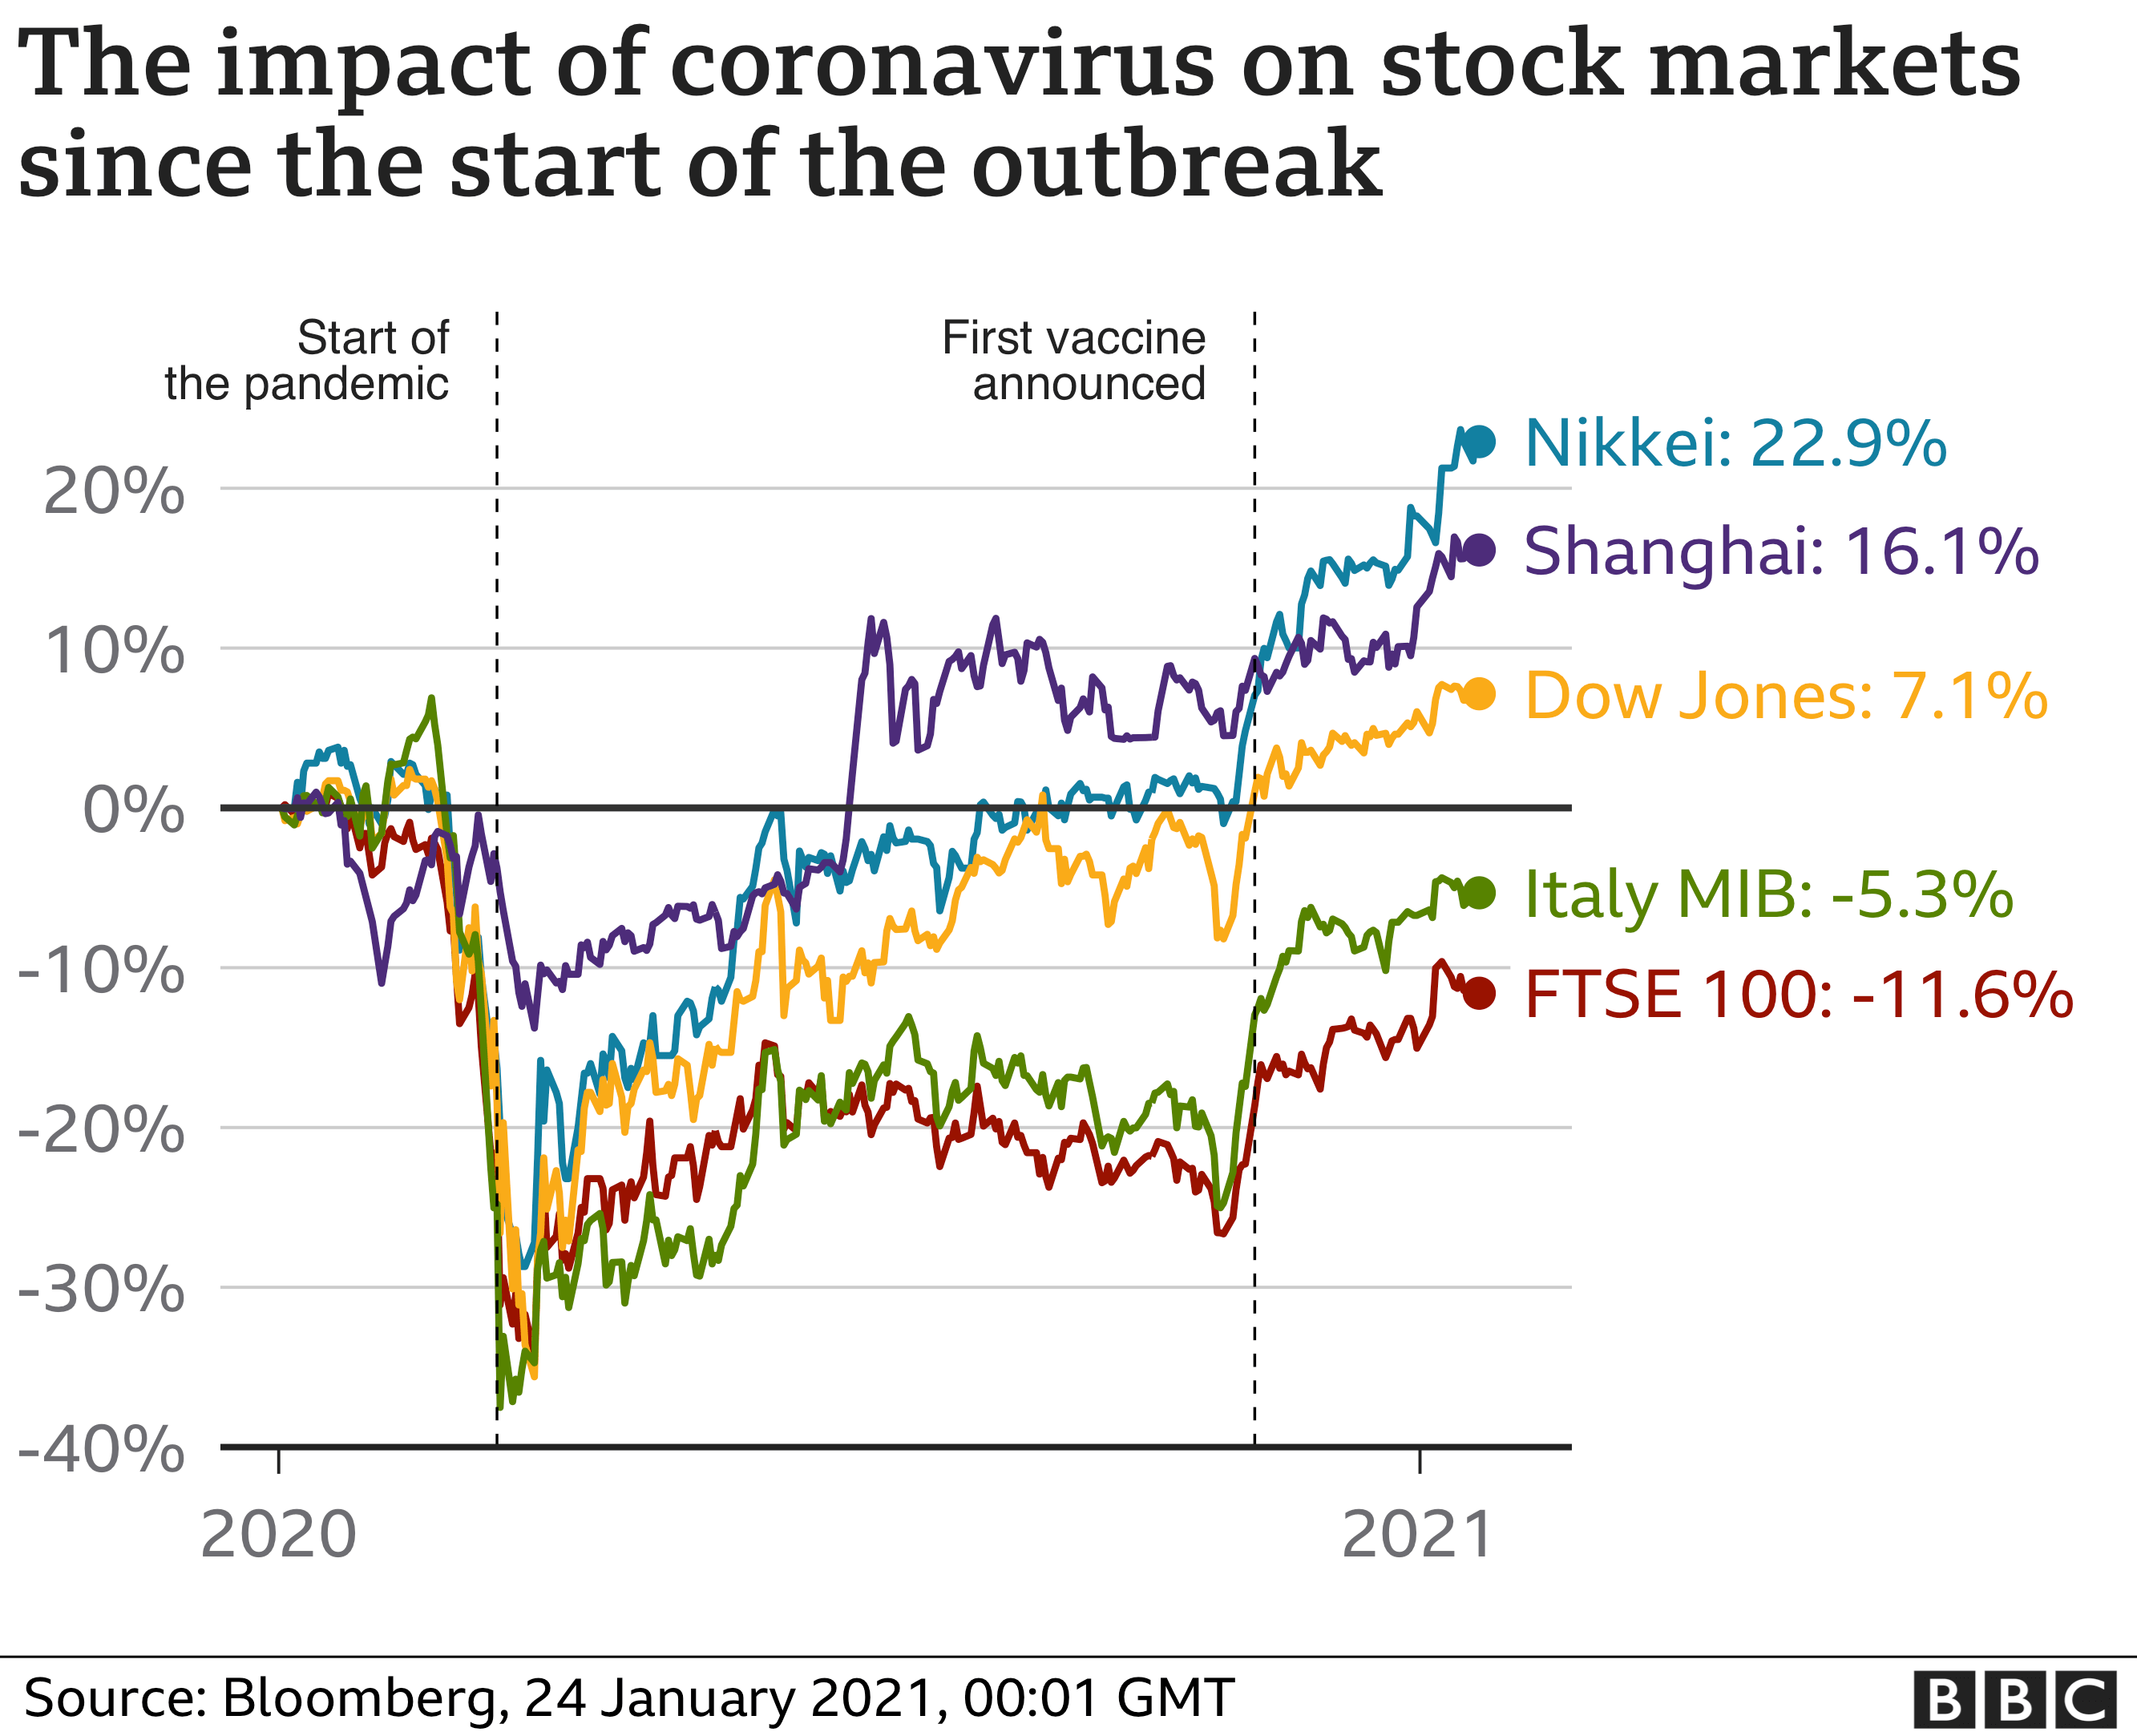
\includegraphics[width=\textwidth]{figures/covid_shock_stocks.png}%
      \caption{The impact of Covid on the stock market. Source: BBC, based on Bloomberg data}%
    \end{figure}
  \end{minipage}%
  \hfill%
  \pause%
  \begin{minipage}{0.47\textwidth}%
    \begin{small}%
      \textbf{Economic impact of unexpected shocks:}%
      \begin{itemize}%
        \item[$\blacktriangleright$] (Long-term) Expectations about new viruses exist.%
        \item[$\blacktriangleright$] However, realization of new viruses is normally unexpected.%
        \pause%
        \item[$\blacktriangleright$] Significant drop in the value of stock markets as Covid unfolds.%
        \item[$\blacktriangleright$] Also, unexpected increase in stock market values as vaccine was introduced.%
      \end{itemize}%
    \end{small}%
  \end{minipage}%
\end{frame}%
%-------------------------------------------------------------------------
% Stochastic Elements: How to model the Russian Invasion on Ukraine?
\begin{frame}{Stochastic Elements: How to model the Russian Invasion of Ukraine?}%
  \begin{minipage}{0.5\textwidth}%
    \begin{figure}%
      \centering%
      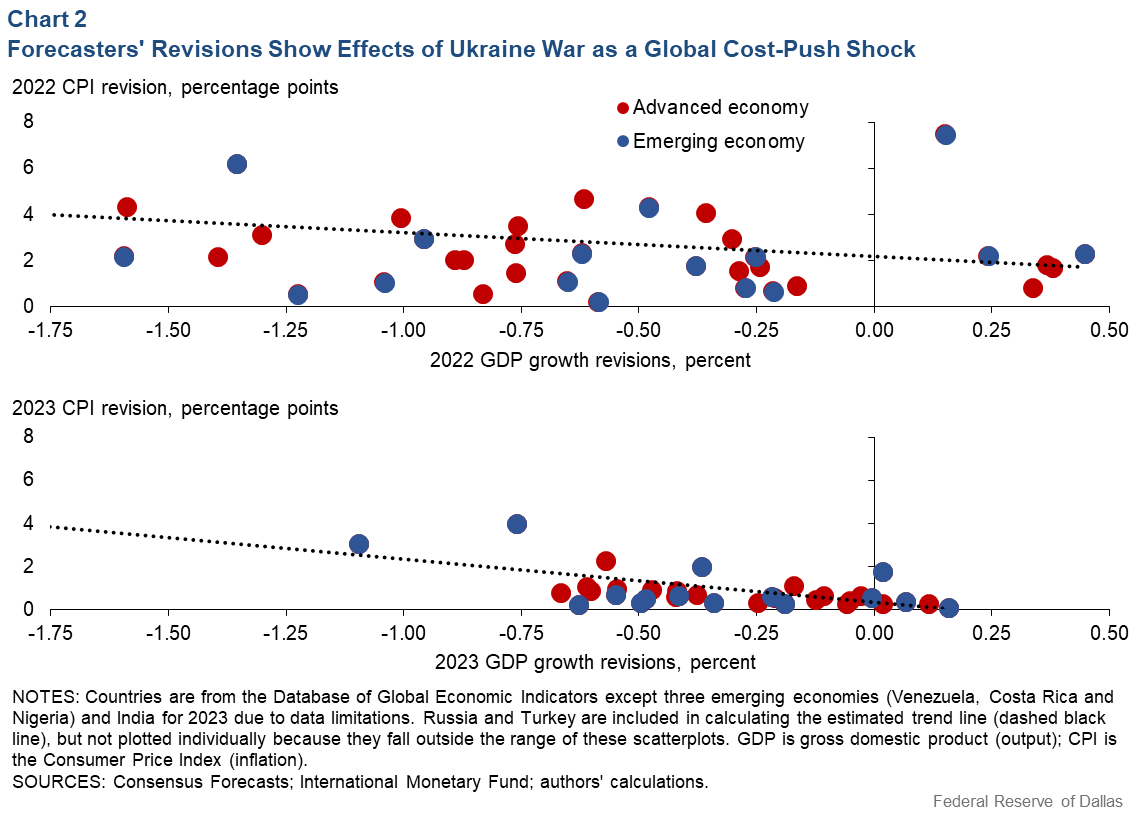
\includegraphics[width=\textwidth]{figures/ukraine_shock_cpi.png}%
      \caption{Forecast revision for inflation and GDP growth after the Russian invasion of Ukraine. Source: Federal Reserve Bank of Dallas (data: Consensus Forecasts, IMF)}%
    \end{figure}%
  \end{minipage}%
  \hfill%
  \pause%
  \begin{minipage}{0.47\textwidth}%
    \begin{small}%
      \textbf{Economic impact of unexpected shocks:}%
      \begin{itemize}%
        \item[$\blacktriangleright$] Widely unexpected event: How did it change the economics of the world?%
        \pause%
        \item[$\blacktriangleright$] How to model this event? Long-term vs short-term change?%
        \item[$\blacktriangleright$] How do the economic dynamics of this shock look like?%
        \pause%
        \item[$\Rightarrow$] Both the dynamic transition of the shock and expectations about future shocks need to be taken into account!%
      \end{itemize}%
    \end{small}%
  \end{minipage}%
\end{frame}%
%-------------------------------------------------------------------------
% Critique of the AS-AD Model - What this Course is about
\begin{frame}{Critique of the AS-AD Model - What this Course is about}%
  \begin{itemize}%
    \item[$\blacktriangleright$] \textbf{Ad-hoc Modeling:} No modeling of the deep/fundamental parameters. Models are not based on economic reasoning, but on statistical correlations.%
    \begin{itemize}%
      \item[$\rightarrow$] \textbf{Lucas (1976) Critique:} Conditional (on policy changes) forecasts need structural models. Estimated regularities break down if policy tries to exploit them.%
    \end{itemize}%
    \pause%
    \item[$\blacktriangleright$] \textbf{Static Model:} Short-, medium-, and long-run are three different models. Transitions are fuzzy and up to idiosyncratic interpretation.%
    \pause%
    \item[$\blacktriangleright$] \textbf{Perfect Foresight:} There is no uncertainty in this model. As there is no explicit time, this is hard to model. Nevertheless, uncertainty is an important driver of business cycles.%
    \vspace{0.1in}%
    \pause%
    \item[$\Rightarrow$] In this course, we learn how to construct Dynamic Stochastic General Equilibrium (DSGE) models, how to simulate them using a computer, and how to conduct policy analysis with those models!%
  \end{itemize}%
\end{frame}%
%-------------------------------------------------------------------------
% BLOCK 1 - Which Topics do we cover in this Course?
%-------------------------------------------------------------------------
\section{Which Topics\\do we cover in this Course?}
%-------------------------------------------------------------------------
% How does Money affect the Macroeconomy?
\begin{frame}{How does Money affect the Macroeconomy?}%
  \begin{minipage}{0.5\textwidth}%
    \begin{figure}%
      \centering%
      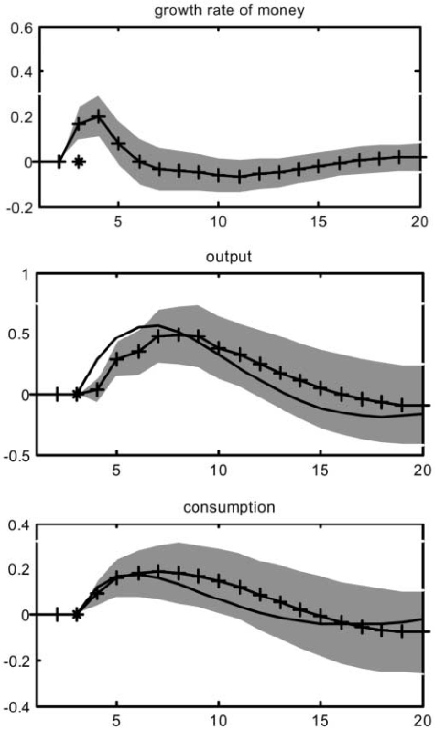
\includegraphics[width=0.6\textwidth]{figures/money_gdp_christiano.png}%
      \caption{Impulse response functions for money, output and consumption Source: Christiano et al. (2005)}%
    \end{figure}%
  \end{minipage}%
  \hfill%
  \pause%
  \begin{minipage}{0.47\textwidth}%
    \begin{small}%
      \textbf{Money drives output in the short-run:}%
      \begin{itemize}%
        \item[$\blacktriangleright$] What are the channels through which money affects the real economy?%
        \item[$\blacktriangleright$] What is the long-run impact of money on the real economy?%
        \item[$\blacktriangleright$] How high is optimal money supply?%
      \end{itemize}%
    \end{small}%
  \end{minipage}%
\end{frame}%
%-------------------------------------------------------------------------
% How should Central Banks set their Interest Rate?
\begin{frame}{How should Central Banks set their Interest Rate?}%
  \begin{minipage}{0.5\textwidth}%
    \begin{figure}%
      \centering%
      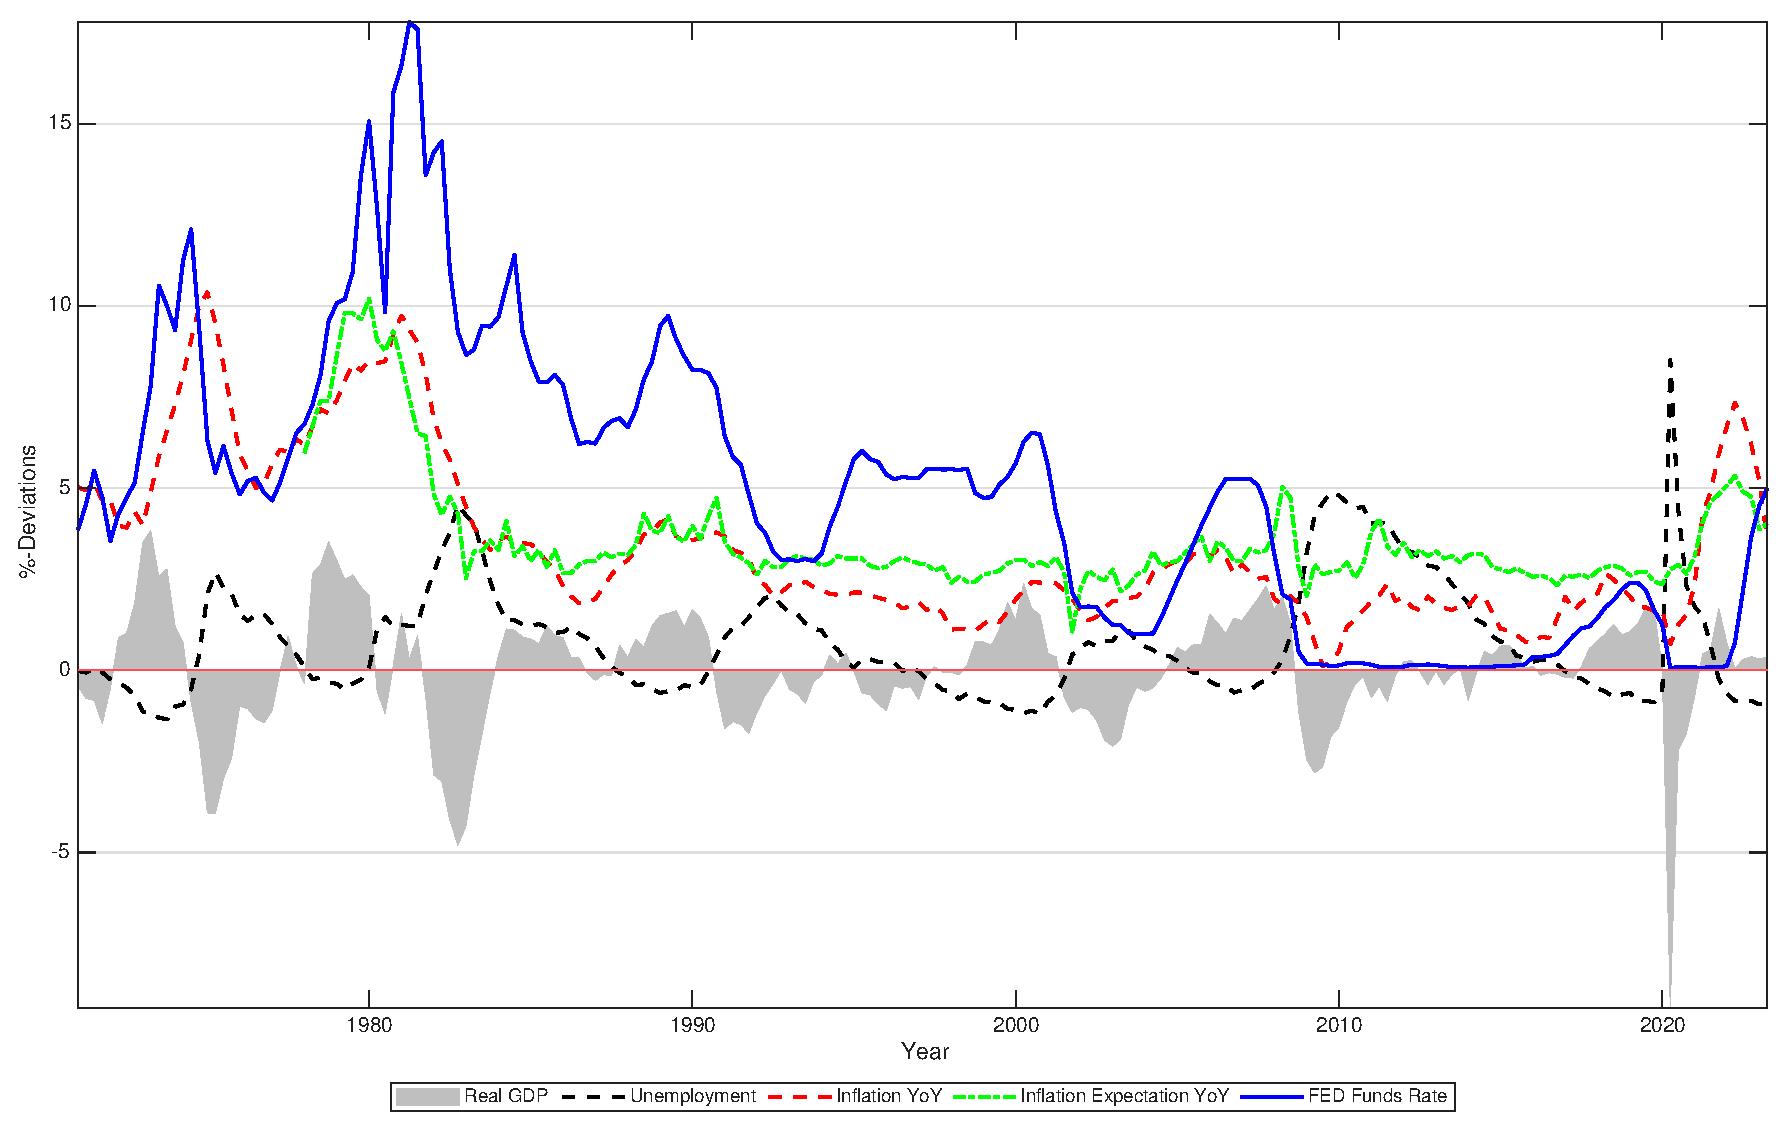
\includegraphics[width=\linewidth]{figures/infl_interest.eps}%
      \vspace*{-0.1in}%
      \caption{FED funds rate and U.S. year-on-year inflation rates, quarterly data (1980-2023).}%
      \vspace*{-0.5in}%
    \end{figure}%
  \end{minipage}%
  \hfill%
  \pause%
  \begin{minipage}{0.47\textwidth}%
    \begin{small}%
      \textbf{Central banks stablize the business cycle:}%
      \begin{itemize}%
        \item[$\blacktriangleright$] What is an appropriate policy target?%
        \item[$\blacktriangleright$] Do people trust their central bank to achieve this target?%
        \item[$\blacktriangleright$] What instruments stabilize the economy best? What are potential tradeoffs?
      \end{itemize}%
    \end{small}%
  \end{minipage}%
\end{frame}%
%-------------------------------------------------------------------------
% What is the Macroeconomic Impact of different Forms of Taxation?
\begin{frame}{What is the Macroeconomic Impact of different Forms of Taxation?}%
  \begin{minipage}{0.5\textwidth}%
    \begin{figure}%
      \centering%
      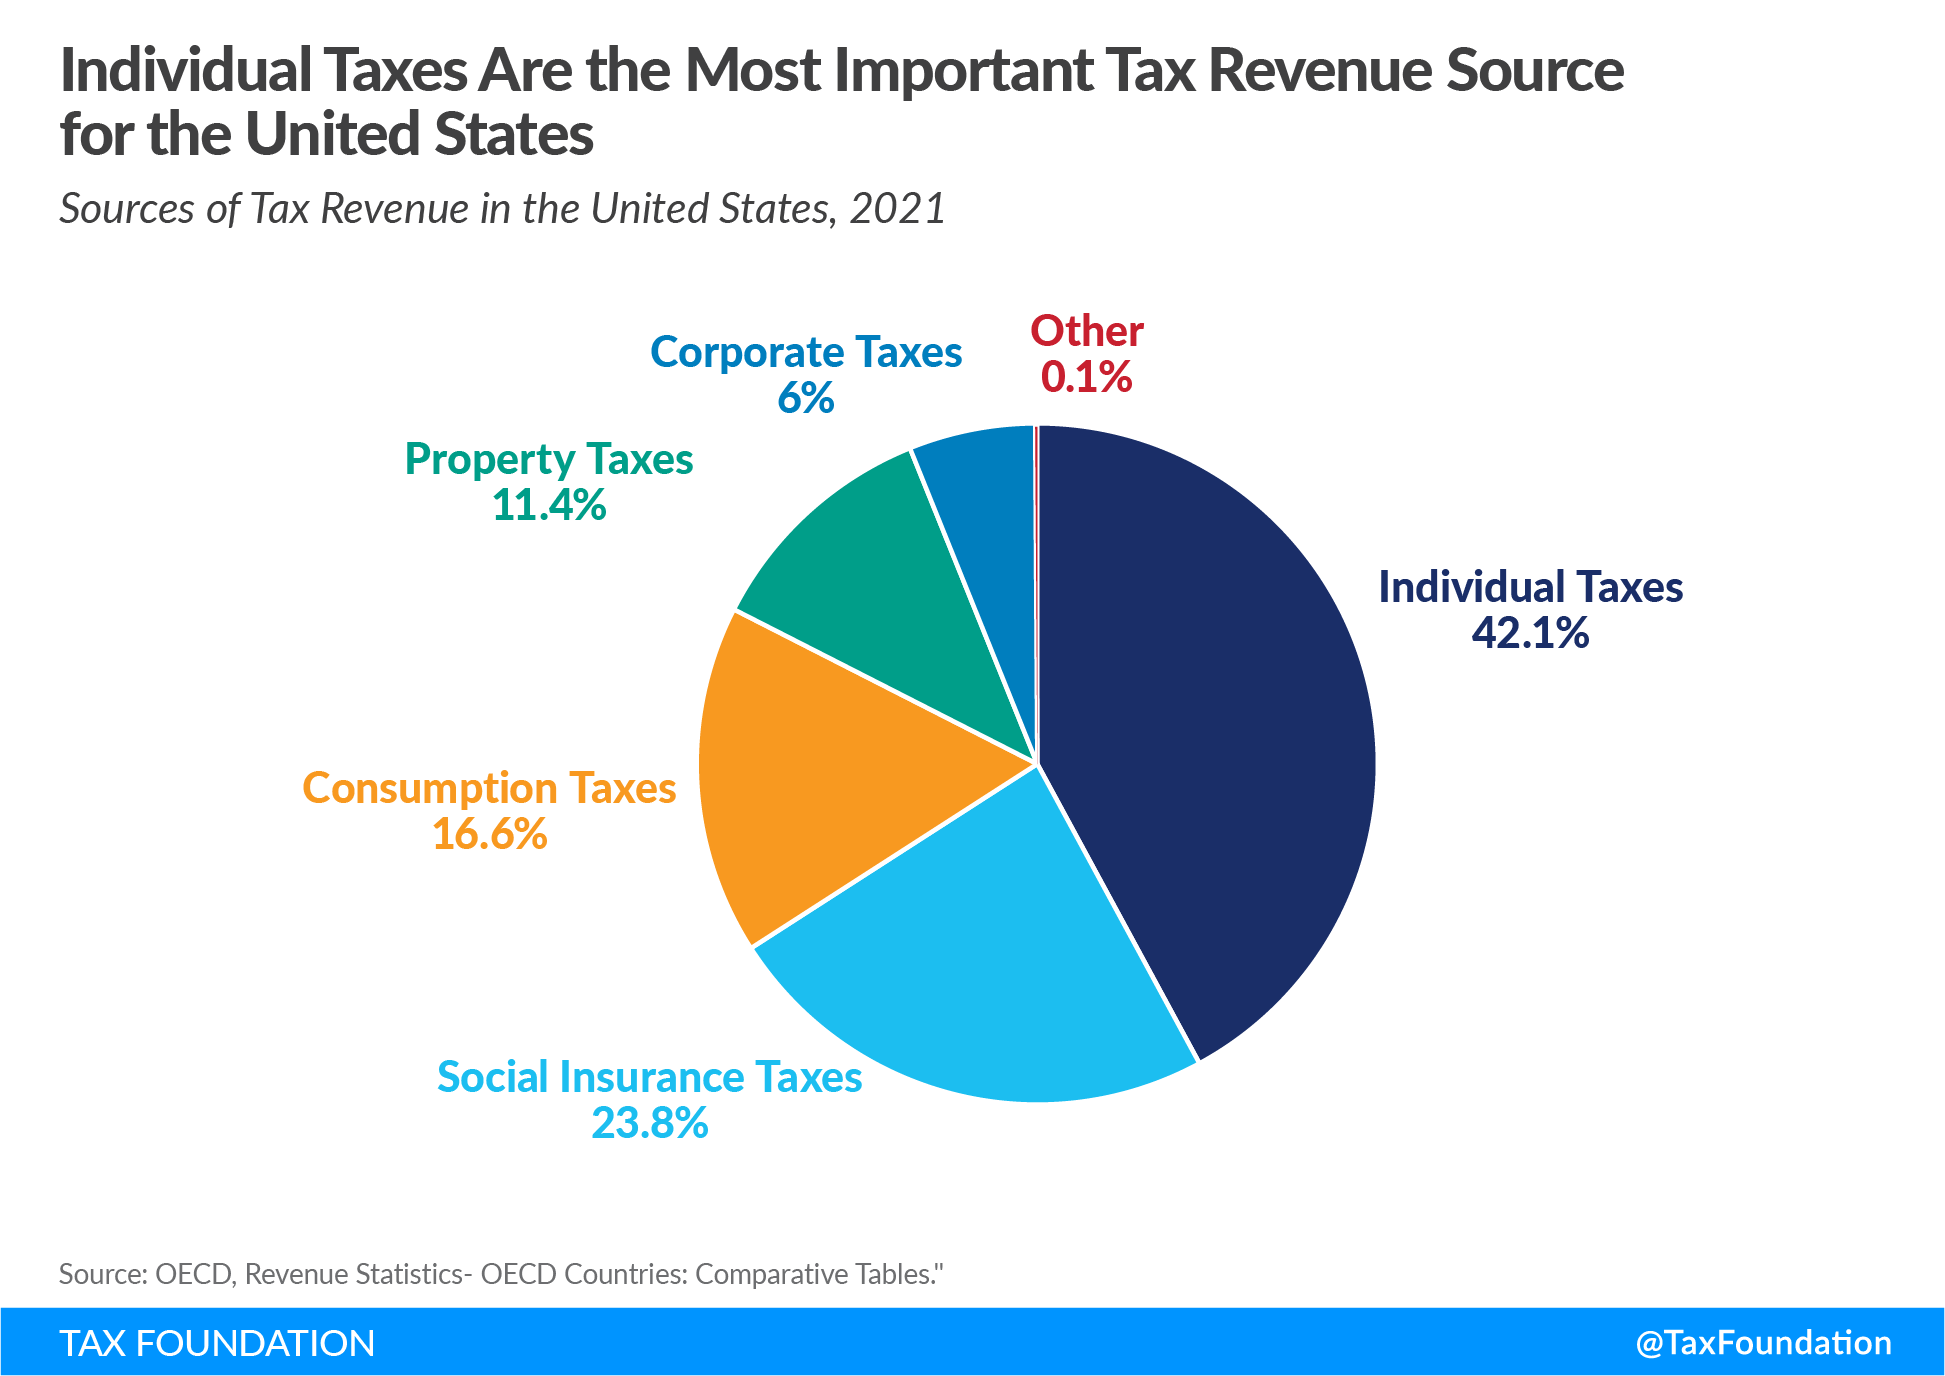
\includegraphics[width=\textwidth]{figures/tax_sources_us.png}%
      \vspace*{-0.1in}%
      \caption{Tax revenue shares in the US (2021). Source: Tax Foundation (data: OECD Revenue Statistics)}%
    \end{figure}%
  \end{minipage}%
  \hfill%
  \pause%
  \begin{minipage}{0.47\textwidth}%
    \begin{small}%
      \textbf{The macroeconomic impact of taxes:}%
      \begin{itemize}%
        \item[$\blacktriangleright$] How should the government raise its tax revenue? 
        \begin{itemize}%
          \item[$\rightarrow$] Individual vs consumption taxes?%
          \item[$\rightarrow$] Capital vs income taxes?%
        \end{itemize}%
        \item[$\blacktriangleright$] What is an optimal amount of overall taxation?%
        \item[$\blacktriangleright$] Do taxes impact business cycle fluctuations?%
      \end{itemize}%
    \end{small}%
  \end{minipage}%
\end{frame}%
% %-------------------------------------------------------------------------
% % BLOCK 2 - Assignment 0: A Basic Approach to Intertemporal Macroeconomics
% %-------------------------------------------------------------------------
% \section{A Basic Approach to Intertemporal Macroeconomics\\\small{Assignment 0}}
%-------------------------------------------------------------------------
% BLOCK 3 - The Cash-in-Advance Model - Basic Setup
%-------------------------------------------------------------------------
\section{The Cash-in-Advance Model\\\small{Basic Setup (Cole (2020) chapter 2)}}
%-------------------------------------------------------------------------
% Money in the Macroeconomic Model
\begin{frame}{How to Introduce Money in a Macroeconomic Model?}%
  In a frictionless world, barter is generally preferred to money as money has no value.\\%
  \medskip%
  \emph{However:}%
  \pause%
  \begin{itemize}%
    \item[$\blacktriangleright$] People cannot track other's identities, hence (long-term) contracts are difficult.%
    \item[$\blacktriangleright$] Trade often is sequential involving people that either want to buy or sell a good.%
    \item[$\Rightarrow$] Barter is not possible, as there is no goods-for-goods exchange anymore.%
    \item[$\Rightarrow$] Money acts as a medium of exhange. \textbf{Simplest friction: Cash-in-Advance (CiA)!}%
  \end{itemize}%
  \vspace*{0.2in}%
  \pause%
  The use of money is here by assumption!%
  \begin{itemize}%
    \item[$\blacktriangleright$] Hence, it is a poor model for understanding the role of money.%
    \item[$\blacktriangleright$] However, the assumption is accurate enough to understand the impact of changes in money supply and other exogenous variables.%
  \end{itemize}%
\end{frame}%
%-------------------------------------------------------------------------
% CiA Model: Basic Structure of the Economy
\begin{frame}{CiA Model: Basic Structure of the Economy}%
  Our model economy consists of different households, firms, and a government:%
  \begin{itemize}%
    \item[$\blacktriangleright$] There are only household-firm pairs, hence no individual firms (for now).%
    \item[$\blacktriangleright$] In each period, a household can produce one of many types of goods, $i \in I$.%
  \end{itemize}%
  \vspace*{0.1in}%
  \pause%
  Each household is composed of two agents: A seller and a buyer.%
  \begin{itemize}
    \item[$\blacktriangleright$] A buyer takes available household cash to buy all the types of goods the household desires.%
    \item[$\blacktriangleright$] A seller tries to sell some of the household good, $i$, saving the rest to consume themselves.%
  \end{itemize}%
  \vspace*{0.1in}%
  \pause%
  The model markets are framed by properties and institutions:%
  \begin{itemize}%
    \item[$\blacktriangleright$] Each goods market $i \in I$ has lots of buyers and sellers $\Rightarrow$ \textbf{markets are competitive!}%
  \end{itemize}%
\end{frame}%
%-------------------------------------------------------------------------
% CiA Model: Goods and Asset Markets
\begin{frame}{CiA Model: Goods and Asset Markets}%
  To keep things simple, we will assume that the supply and demand of goods is symmetric:%
  \begin{itemize}%
    \item[$\blacktriangleright$] All prices, $P(i)$, that clear these markets will be identical.%
  \end{itemize}%
  \bigskip%
  \pause%
  There is an asset market where households exchange money and financial assets:%
  \begin{itemize}%
    \item[$\blacktriangleright$] We assume that the only type of asset is a one-period pure discount bond.%
    \item[$\blacktriangleright$] The presence of this bond will give us an interest rate that we can determine.%
    \item[$\blacktriangleright$] Monetary policy is conducted by changing the money supply or through the bonds market.%
  \end{itemize}%
\end{frame}%
%-------------------------------------------------------------------------
% CiA Model: Production and Utility
\begin{frame}{CiA Model: Production and Utility}%
  \textbf{Production function:}%
  \begin{itemize}%
    \item[$\blacktriangleright$] Each household produces the good at the beginning of each period by%
    \begin{align}%
      y_{i}=ZL,  \label{production function}%
    \end{align}%
    where $Z>0$ is productivity of the economy, and $L\geq 0$ is household hours worked.%
  \end{itemize}%
  \bigskip%
  \pause%
  \textbf{Utility function:}%
  \begin{itemize}%
    \item[$\blacktriangleright$] Each household has the following preferences over its consumption in a period:%
    \begin{align}%
      u(C)\text{ concave},\text{ and }C=\left\{ \frac{1}{\#I}\sum_{i\in I}C(i)^{\rho }\right\}^{1/\rho},  \label{cons preferences}%
    \end{align}%
    where $\#I$ is the number of different goods and $\rho \in (0,1)$ defines their substitutability.%
    \item[$\blacktriangleright$] A concave utility function implies $u^{\prime}(C)>0$ and $u^{\prime \prime}(C)<0$.%
  \end{itemize}%
\end{frame}%
%-------------------------------------------------------------------------
% CiA Model: Labor Disutility and Payoff
\begin{frame}{CiA Model: Labor Disutility and Payoff}%
  \textbf{Labor disutility:}%
  \begin{itemize}%
    \item[$\blacktriangleright$] Household preferences over labor supply in a period are given by $v(L)$.%
    \item[$\blacktriangleright$] $v(L)$ is convex; specifically it follows that $v^{\prime }>0$ and $v^{\prime \prime }>0.$%
    \item[$\blacktriangleright$] The cost of additional labor effort is positive and increasing in its level.%
  \end{itemize}%
  \vspace*{0.2in}%
  \pause%
  \textbf{Household payoff function:}%
  \begin{itemize}%
    \item[$\blacktriangleright$] The total payoff per period for a household is given by%
    \begin{align}%
      \mathbb{U} \; = \; u(C) - v(L).  \label{static prreferences}%
    \end{align}%
    \item[$\blacktriangleright$] Overall utility increases in consumption and decreases in labor effort!%
  \end{itemize}%
\end{frame}%
%-------------------------------------------------------------------------
% CiA Model: Timing
\begin{frame}{CiA Model: Timing}%
  \begin{center}%
  \begin{tabular}{l}%
    \textbf{Timing within each period} \\%
    \\%
    \pause%
    1. The household starts a period with $M$ units of money.\\%
    \pause%
    2. It exerts labor effort $L$ to produce its good.\\%
    \pause%
    3. The seller and buyer split up and go to their respective markets.\\%
    \pause%
    4. The seller and buyer come back together in the asset market.\\%
    \pause%
    5. They jointly consume the consumption good.\\%
    \pause%
    6. The period ends.%
  \end{tabular}\\%
  \vspace*{0.3in}%
  \pause%
  $\Rightarrow$ The timing of the model \emph{will end up mattering quite a bit.}%
  \end{center}%
\end{frame}%
%-------------------------------------------------------------------------
% BLOCK 2 - The Cash-in-Advance Model - Static Version
%-------------------------------------------------------------------------
\section{The Cash-in-Advance Model\\\small{Static Version (Cole (2020) chapter 2)}}
%-------------------------------------------------------------------------
% Starting Point and Simplification
\begin{frame}{Starting Point and Simplification}%
  \begin{block}{Simplification:}%
    Static version of the household's problem, hence we will only look at the current period taking the future as given (we move to the dynamic version later on)!%
  \end{block}%
  \vspace*{0.1in}%
  \pause%
  \textbf{Properties of the static model:}%
  \begin{itemize}%
    \item[$\blacktriangleright$] Denote by $V(W)$ the future value of wealth, $W$.%
    \item[$\blacktriangleright$] We do not yet distinguish among the types of wealth.%
    \item[$\blacktriangleright$] We use continuation payoff functions to avoid infinite horizon models.%
  \end{itemize}%
  \vspace*{0.1in}%
  \pause%
  The household can be thought of as choosing {\footnotesize(control variables!)} how much%
  \begin{itemize}%
    \item[$\blacktriangleright$] to consume of each of the different goods, $\left\{ C(i)\right\} _{i\in I}$,%
    \item[$\blacktriangleright$] to work to produce their production good, $L(j)$,%
    \item[$\blacktriangleright$] wealth, $W$, for next period in order to maximize its payoff.%
  \end{itemize}%
\end{frame}%
%-------------------------------------------------------------------------
% Household Utility Maximization
\begin{frame}{Household Utility Maximization}%
  Formalization of the \textbf{optimization problem} for a household whose production type is $j$:%
  \begin{align*}%
    \max_{\left\{ C(i)\right\} _{i\in I},L(j),W}\ u(C)-v(L(j))+V(W)%
  \end{align*}%
  subject to%
  \pause%
  \begin{itemize}%
    \item[$\blacktriangleright$] a \textbf{cash-in-advance condition}, which states that the household can only spend as much as it has in cash to buy goods (the notation $I/j$ means the set $I$ less element $j$.):%
    \begin{align*}%
      M \geq \sum_{i\in I/j}P(i)C(i)
    \end{align*}%
    \pause%
    \item[$\blacktriangleright$] a \textbf{budget constraint}, which states that the household's net period wealth is whatever it has left out of its money holdings and the proceeds of what it sells in the goods market:%
    \begin{align*}%
      W \leq P(j)\left[ ZL(j)-C(j)\right] +\left[ M-\sum_{i\in I/j}P(i)C(i)\right]%
    \end{align*}%
  \end{itemize}%
\end{frame}%
%-------------------------------------------------------------------------
% Lagrangian of the Household Utility Maximization
\begin{frame}{Lagrangian of the Household Utility Maximization}%
  To address this multi-dimensional maximization problem, we \textbf{form the Lagrangian:}%
  \begin{eqnarray}%
    \mathcal{L} &=&\max_{\left\{ C(i)\right\} _{i\in I},L(j),W}\min_{\lambda,\mu }\ u(C)-v(L(j))+V(W)  \label{Lagrangian 1} \\%
    &&+\lambda \left\{ M-\sum_{i\in I/j}P(i)C(i)\right\}  \notag \\%
    &&+\mu \left\{ P(j)\left[ ZL(j)-C(j)\right] +\left[ M-\sum_{i\in I/j}P(i)C(i)\right] -W\right\} .  \notag%
  \end{eqnarray}\\%
  \vspace*{0.2in}%
  \pause%
  $\lambda $ and $\mu $ are the \textbf{"penalty prices"} that we attach to violations of the constraints:%
  \begin{itemize}%
    \small%
    \item[$\blacktriangleright$] The impact of the penalties comes through violations of the conditions, and can be minimized by setting them so there is no violation. % 
    \item[$\blacktriangleright$] In this maximization we are simultaneously trying to minimize the impact of these penalty prices on the overall objective and maximize the value of the objective in terms of the direct choice variables.%
  \end{itemize}%
\end{frame}%
%-------------------------------------------------------------------------
% First-Order Conditions for Consumption
\begin{frame}{First-Order Conditions for Consumption}%
  The \textbf{first-order conditions (FOCs)} will include the consumption conditions for each type of consumption, or%
  \begin{align*}%
    u^{\prime }(C)\left\{ \frac{1}{\#I}\sum_{i}C(i)^{\rho }\right\} ^{(1-\rho)/\rho }\frac{1}{\#I}C(i)^{\rho -1} \; = \; \left( \lambda +\mu \right) P(i)%
  \end{align*}%
  for each $i\neq j$.\\%
  \medskip%
  \pause%
  For their own good $j,$ the condition is%
  \begin{align*}%
    u^{\prime }(C)\left\{ \frac{1}{\#I}\sum_{i}C(i)^{\rho }\right\} ^{(1-\rho)/\rho }\frac{1}{\#I}C(j)^{\rho -1}=\mu P(j).%
  \end{align*}%
  \pause%
  \begin{itemize}%
    \small%
    \item[$\blacktriangleright$] Note that this implies that the household will consume more of its own good to the extent that the cash-in-advance constraint binds and $\lambda >0. $%
    \item[$\blacktriangleright$] This pattern arrises because holding money has a cost due to its poor return.%
  \end{itemize}%
\end{frame}%
%-------------------------------------------------------------------------
% First-Order Conditions for Labor and Wealth
\begin{frame}{First-Order Conditions for Labor and Wealth}%
  \textbf{Optimal condition for labor effort}:%
  \begin{align}%
    v^{\prime }(L(j)) \; = \; \mu P(j)Z.  \label{pricing eq good j}%
  \end{align}\\%
  \vspace*{0.2in}%
  \pause%
  \textbf{Optimal choice of wealth:}%
  \begin{align}%
    V^{\prime }(W) \; = \; \mu .%
  \end{align}\\%
  \vspace*{0.2in}%
  \pause%
  We can use this last result to replace $\mu$ in the consumption and labor conditions.%
  \normalsize%
\end{frame}%
%-------------------------------------------------------------------------
% BLOCK 2 - The Cash-in-Advance Model - Symmetric Goods Market
%-------------------------------------------------------------------------
\section{The Cash-in-Advance Model\\\small{Symmetric Goods Market (Cole (2020) chapter 2)}}
%-------------------------------------------------------------------------
% Modification of CiA Constraint
\begin{frame}{Modification of CiA Constraint}%
  \begin{block}{Simplifying Modification}%
    \small%
    Going forward, we will not be interested in the extent to which households buy more of their own good because they don't need to use cash. Focus a model on what you want to study. Detail for details sake is bad.%
  \end{block}%
  \pause%
  Assume that you have to use cash even to buy your own consumption good. So, the constraints become%
  \begin{align*}%
    M \; \geq \; \sum_{i\in I}P(i)C(i)%
  \end{align*}%
  and%
  \begin{align*}%
    W \; \leq \; P(j)ZL(j)+\left[ M-\sum_{i\in I}P(i)C(i)\right] .%
  \end{align*}%
\end{frame}%
%-------------------------------------------------------------------------
% Symmetric Prices across Goods
\begin{frame}{Symmetric Prices across Goods}%
  \begin{small}%
    Given that the prices of the consumption good are the same $P(i)=\tilde{P}$ and $C(i)=C$:%
    \pause%
    \begin{itemize}%
      \item[$\blacktriangleright$] The derivative of the inside aggregator w.r.t. $C(i) $ is given by:%
      \begin{align*}
        \left\{ \frac{1}{\#I}\sum_{i}C(i)^{\rho }\right\} ^{(1-\rho )/\rho}C(i)^{\rho -1} \; = \; \left\{ \frac{1}{\#I}\#I\right\} ^{(1-\rho )/\rho}\left\{ C^{\rho }\right\} ^{(1-\rho )/\rho }C^{\rho -1} \\%
        = \; \left\{ C^{\rho }\right\} ^{(1-\rho )/\rho }C^{\rho -1} \; = \; C^{0}=1%
      \end{align*}
      \vspace*{-0.2in}%
      \pause%
      \item[$\blacktriangleright$] Then, note that if you buy $dC$ of each of our consumption goods,  the increase in the composite is also $dC$, and if all of the prices are the same, and the change in $\mathcal{L}$ is:%
      \begin{align*}%
        \sum_{i}u^{\prime }(C)\frac{1}{\#I}dC \; = & \; \sum_{i}\left( \lambda +\mu \right) \tilde{P}dC\text{ or } \\%
        u^{\prime }(C) \; = & \; \left( \lambda +\mu \right) \#I \ast \tilde{P}%
      \end{align*}%
      \vspace*{-0.2in}%
      \pause%
      \item[$\blacktriangleright$] Denote the price of a unit of the composite good (which means one of each individual good) by $P=\#I\tilde{P}$. It follows:%
      \begin{align}%
        u^{\prime }(C) \; = \; \left( \lambda +\mu \right) P  \label{foc cons A}%
      \end{align}%
    \end{itemize}%
  \end{small}%
\end{frame}%
%-------------------------------------------------------------------------
% Binding CiA Constraint and Penalty Prices
\begin{frame}{Binding CiA Constraint and Penalty Prices}%
  If the cash-in-advance constraint \emph{does not bind}, then $\lambda =0$, and%
  \begin{align}%
    u^{\prime }(C) \; = \; V^{\prime }(W)P,  \label{foc cons A1}%
  \end{align}\\%
  \vspace*{0.25in}%
  \pause%
  If the cash-in-advance constraint \emph{does bind}, then $\lambda >0,$%
  \begin{align}%
    C \; = \; \frac{M}{P},  \label{foc cons A2}%
  \end{align}%
  and $\lambda $ will be chosen so that%
  \begin{align*}%
    \lambda \; = \; \frac{u^{\prime }(C)}{P}-V^{\prime }(W).%
  \end{align*}%
\end{frame}%
%-------------------------------------------------------------------------
% Optimal Labor Allocation in the Symmetric Equilibrium
\begin{frame}{Optimal Labor Allocation in the Symmetric Equilibrium}%
    By again using the FOC for wealth, we get a \textbf{optimal choice of labor:}% 
    \begin{align}%
      v^{\prime }(L(j)) \; = \; V^{\prime }(W)P(j)Z,  \label{foc labor A}%
    \end{align}%
    which says that the optimal labor choice is to set the marginal disutility of effort equal to the nominal marginal labor product, $P(j)Z,$ times the marginal value of nominal wealth, $V^{\prime }(W)$.\\%
    \vspace*{0.3in}%
    \pause%
    We want to \emph{rewrite this in terms of the composite price}:%
    \begin{align*}%
      v^{\prime }(L(j)) \; = \; V^{\prime }(W)PZ/\#I.%
    \end{align*}%
    \pause%
    Then if we change $Z$ to $Z\ast \#I,$ we get%
    \begin{align*}%
      v^{\prime }(L)=V^{\prime }(W)PZ.%
    \end{align*}%
\end{frame}%
%-------------------------------------------------------------------------
% BLOCK 2 - The Cash-in-Advance Model - Asset Markets
%-------------------------------------------------------------------------
\section{The Cash-in-Advance Model\\\small{Asset Markets (Cole (2020) chapter 2)}}
%-------------------------------------------------------------------------
% Introducing the Asset Market
\begin{frame}{Introducing the Asset Market}%
  We now extend our simple model to incorporate an asset market at the end of the period:%
  \pause%
  \begin{itemize}%
    \item[$\blacktriangleright$] Households can exchange money for bonds and vice versa.%
    \pause%
    \item[$\blacktriangleright$] Households can buy and sell government bonds, which are just another form of bond.%
    \pause%
    \item[$\blacktriangleright$] We now have to distinguish between two types of wealth: Money and bonds!%
    \begin{itemize}%
      \item[$\rightarrow$] Next period's money and bond positions are denoted by $B^{\prime}$ and $M^{\prime}$.%
      \item[$\rightarrow$] Future household payoff is denoted by $V(B^{\prime}, M^{\prime})$.%
    \end{itemize}%
    \pause%
    \item[$\blacktriangleright$] All bonds are pure discount bonds:%
    \begin{itemize}%
      \item[$\rightarrow$] The payoff is \$ 1 for each unit of the bond and the cost is $q$ per unit today.%
      \item[$\rightarrow$] Note that $\frac{1}{q} = R$ is the gross interest rate offered by the bond.%
    \end{itemize}%
  \end{itemize}%
\end{frame}%
%-------------------------------------------------------------------------
% Asset Market Lagrangian
\begin{frame}{Asset Market Lagrangian}%
  The household faces a \textbf{budget constraint} in the bond market, which we can write as%
  \begin{align*}%
    P Z L + \left[ M - PC \right] + B \; \geq \; M^{\prime} + q B^{\prime}.%
  \end{align*}\\%
  \vspace*{0.25in}%
  \pause%
  With these changes we can \textbf{rewrite its Lagrangian} as%
  \begin{align*}%
    \mathcal{L} \; = \; \max_{\left\{ C(i)\right\} _{i\in I},L(j),M^{\prime},B^{\prime }} \min_{\lambda ,\mu} & \; u(C) - v(L(j)) + V(M^{\prime}, B^{\prime})\label{Lagrangian 2}\\%
    & \; + \lambda \left\{ M - P C \right\}\notag\\%
    & \; + \mu \left\{ P Z L + \left[ M - P C \right] + B - M^{\prime} - q B^{\prime}\right\}. \notag%
  \end{align*}%
\end{frame}%
%-------------------------------------------------------------------------
% Static CiA Model: Asset Market First-Order Conditions
\begin{frame}{Static CiA Model: Asset Market First-Order Conditions}%
  The \textbf{FOC for money}, $M^{\prime}$, is%
  \begin{align*}%
    -\mu + V_{1}(M^{\prime}, B^{\prime}) \; = \; 0.%
  \end{align*}%
  \pause%
  Similarly, the \textbf{FOC for bonds}, $B^{\prime}$, is%
  \begin{align*}%
    -\mu q + V_{2}(M^{\prime}, B^{\prime}) \; = \; 0,%
  \end{align*}%
  \medskip\\%
  \pause%
  These two conditions differ in important ways.%
  \begin{itemize}%
    \item[$\blacktriangleright$] Bonds are cheaper per unit of future value to the extent that $q<1.$%
    \item[$\blacktriangleright$] They contribute future value in different ways to the extent that money and bonds in the future are imperfect substitutes.%
    \item[$\blacktriangleright$] To determine how their future value differs, we need to move on to a \emph{genuine dynamic version of the model} $\rightarrow$ \textbf{next lecture!}%
  \end{itemize}%
\end{frame}%
%-------------------------------------------------------------------------
% CONCLUSION
%-------------------------------------------------------------------------
\section{Conclusion}%
%-------------------------------------------------------------------------
% Summarizing the Lecture
\begin{frame}{Summarizing the Lecture}%
  \begin{center}%
    \begin{large}%
      Can you summarize the three main aspects of the lecture?%
    \end{large}%
  \end{center}%
\end{frame}%
%-------------------------------------------------------------------------
% Concluding Remarks
\begin{frame}{Concluding Remarks}%
  \begin{block}{Big Picture of the Lecture}%
    \begin{enumerate}%
      \item Why do we need dynamic macroeconomic models to explain business cycle fluctuations?%
      \item How do we go from microeconomics to aggregate macroeconomic models?%
    \end{enumerate}%
  \end{block}%
  \pause%
  \vspace*{0.2in}%
  We started out by criticizing older macroeconomic models. In particular:
  \begin{itemize}%
    \item[$\blacktriangleright$] \textbf{Ad-hoc Modeling:} We have started to use micro-founded macroeconomics where the starting point is each single household and firm.%
    \pause%
    \item[$\blacktriangleright$] \textbf{Static Models:} We will introduce dynamic models in the second lecture.%
    \pause%
    \item[$\blacktriangleright$] \textbf{Perfect Foresight:} We will introduce random processes and expectations in the third lecture.%
  \end{itemize}%
\end{frame}%
%-------------------------------------------------------------------------
% REFERENCES AND APPENDIX
\appendix%
\begin{frame}{References}%
  \begin{footnotesize}%
    \begin{itemize}%
      \item[$\blacktriangleright$] Burda, M. and Charles W. (2022). Macroeconomics: A European Text. 8th Edition. Oxford University Press.%
      \item[$\blacktriangleright$] Cole, H. L. (2020). Monetary and Fiscal Policy through a DSGE Lens. Oxford University Press.%
      \item[$\blacktriangleright$] Jones, C. I. (2020). Macroeconomics: International Student Edition. 5th Edition. Norton \& Company.%
      \item[$\blacktriangleright$] Lucas Jr, R. E. (1976, January). Econometric policy evaluation: A critique. In Carnegie-Rochester conference series on public policy (Vol. 1, pp. 19-46). North-Holland.%
      \item[$\blacktriangleright$] Phillips, A. W. (1958). The Relation between Unemployment and the Rate of Change of Money Wage Rates in the United Kingdom 1861-1957. Economica 283.%
      \item[$\blacktriangleright$] FRED Economic Data. St Louis FED. Data retrived on. \href{https://fred.stlouisfed.org/}{https://fred.stlouisfed.org/}%
      \begin{itemize}%
        \begin{scriptsize}%
          \item[$\rightarrow$] Real gross domestic product. Code: GDPC1%
          \item[$\rightarrow$] Nominal gross domestic product. Code: GDP%
          \item[$\rightarrow$] Real private investment. Code: GPDIC1%
          \item[$\rightarrow$] Real private consumption. Code: PCECC96%
          \item[$\rightarrow$] Real government consumption expenditures and gross investment. Code: GCEC1%
          \item[$\rightarrow$] Unemployment rate. Code: UNRATE%
          \item[$\rightarrow$] Natural unemployment rate. Code: NROU%
          \item[$\rightarrow$] NBER based recessions indicator. Code: USREC%
          \item[$\rightarrow$] University of Michigan: Inflation expectation. Code: MICH%
          \item[$\rightarrow$] Federal funds effective rate. Code: FEDFUNDS%
          \item[$\rightarrow$] Core PCE inflation (year-on-year). Code: BPCCRO1Q156NBEA%
        \end{scriptsize}%
      \end{itemize}%
  \end{itemize}%
  \end{footnotesize}%
\end{frame}%
%-------------------------------------------------------------------------
\end{document}%